\documentclass[titlepage]{article}

\usepackage[margin=1in,a4paper]{geometry}
% \usepackage[
%   a4paper,
%   total={170mm,257mm},
%   left=20mm,
%   top=20mm
% ]{geometry}

% Header
\usepackage{fancyhdr}
\pagestyle{fancy}
\fancyhead{}
\fancyfoot{}
\renewcommand{\headrulewidth}{0.4pt}
\fancyhead[L]{PPI1-Molla}
\fancyhead[R]{\thepage}

% Equations
\setlength{\jot}{8pt}

% Tables
\renewcommand{\arraystretch}{1.2}
\setlength{\tabcolsep}{10pt}

\usepackage[italian]{babel}
\usepackage[T1]{fontenc}
\usepackage[utf8]{inputenc}
\usepackage{hyperref}
\usepackage{microtype}

% Math
\usepackage{amsmath,amssymb,amsthm}
\usepackage{diffcoeff}
\usepackage{mathtools}
% \usepackage{cancel}
\numberwithin{equation}{section}
\numberwithin{figure}{section}
\numberwithin{table}{section}

% Physics
% \usepackage{physics}
\usepackage{siunitx}
\sisetup{range-phrase=-,range-units=single}

\usepackage{booktabs}
\usepackage{graphicx}

% \usepackage{tikz}
% \usetikzlibrary{patterns,decorations.pathmorphing}

\title{Sapienza Università di Roma\\[1ex]Laboratorio di Meccanica\\[1ex]PPI1-Molla}
\author{Giulio Russo}
\date{6 maggio 2021}


%


\begin{document}

\maketitle
\tableofcontents

\pagebreak
%%%%%%%%%%%%%%%%%%%%%%%%%%%%%%%
\section{Scopo dell'esperienza}

\begin{itemize}
  \item Eseguire misure dirette di massa, lunghezza e tempo.
  \item Misura della costante elastica di una molla.
  \item Misura dell'accelerazione di gravità.
\end{itemize}

%%%%%%%%%%%%%%%%%%%%%%%%%%%%%%%
\section{Apparato sperimentale}

\begin{itemize}
  \item Una molla appesa ad un supporto con carta millimetrata per effettuare misure di allungamento.
  \item Una bilancia digitale per la misura dei dischetti.
  \item Un cronometro a lettura digitale per le misure di periodo.
  \item Una squadra per ridurre l'errore di parallasse nella misura di allungamento.
\end{itemize}

%--------------------
\subsection{Campioni}

\begin{itemize}
  \item 10 dischetti che si possono appendere alla molla.
\end{itemize}

%-----------------------------------
\subsection{Accorgimenti e consigli}

\begin{itemize}
  \item Attenzione a non allungare eccessivamente la molla rispetto alle condizioni di equilibrio per la misura di periodo (circa \SIrange{1}{1.5}{\centi\metre}).
  \item Fare attenzione che la molla non urti la parte superiore quando è al minimo della lunghezza in quanto altera le misure di periodo.
  \item Assicurasi che le oscillazioni della molla siano, per quanto possibile, verticali e unidimensionali.
\end{itemize}

%-------------------------------
\subsection{Strumenti di misura}

In Tabella~\ref{tab:strumenti} sono riassunte le caratteristiche degli strumenti usati.

\begin{itemize}
  \item \textbf{Bilancia di precisione}.
    La risoluzione è pari a \SI{0.1}{\gram}.
    L'incertezza di tipo B associata alla risoluzione dello strumento è quindi
    $\frac{\text{RIS}}{\sqrt{12}} = \frac{\SI{0.1}{\gram}}{\sqrt{12}} = \SI{0.03}{\gram}$.

    La portata è pari a \SI{3}{\kilogram}.
    Eseguendo la misura di massa nulla il valore mostrato sul display è esattamente zero; si assume quindi che l'offset dello strumento sia trascurabile.

  \item \textbf{Cronometro}.
    La risoluzione è pari a \SI{0.01}{\second}.
    L'incertezza di tipo B associata alla risoluzione dello strumento è quindi
    $\frac{\text{RIS}}{\sqrt{12}} = \frac{\SI{0.01}{\second}}{\sqrt{12}} = \SI{0.003}{\second}$.

  \item \textbf{Carta millimetrata}.
    La risoluzione è pari a \SI{1}{\milli\metre}.
    L'incertezza di tipo B associata alla risoluzione dello strumento è quindi
    $\frac{\text{RIS}}{\sqrt{12}} = \frac{\SI{0.001}{\metre}}{\sqrt{12}} = \SI{0.0003}{\metre}$.

    La portata è pari a \SI{28}{\centi\metre}. L'offset dello strumento è trascurabile.
\end{itemize}

\begin{table}[ht]
  \centering
  \begin{tabular}{lcccc}
    \toprule
    Strumento & Portata & Risoluzione & $\sigma_B$ & Offset \\
    \midrule
    Bilancia di precisione & \SI{3}{\kilogram} & \SI{0.1}{\gram} & \SI{0.03}{\gram} & - \\
    Cronometro & - & \SI{0.01}{\second} & \SI{0.003}{\second} & - \\
    Carta millimetrata & \SI{28}{\centi\metre} & \SI{1}{\milli\metre} & \SI{0.3}{\milli\metre} & - \\
    \bottomrule
  \end{tabular}
  \caption{Caratteristiche degli strumenti usati e incertezze associate alla singola misura. Sono inoltre riportati gli eventuali fattori correttivi di offset e di scala.}
  \label{tab:strumenti}
\end{table}

%%%%%%%%%%%%%%%%%%%%%%%%%%%%%
\section{Strategia di misura}

%-----------------
\subsection{Molla}

Un corpo di massa $M$ soggetto alla sola forza elastica segue la legge di Hooke in una dimensione:
\begin{align}
  F &= -k \Delta x \nonumber \\
  M \ddot{x} &= -k(x - x_0)
\end{align}
con $k$ costante elastica della molla e $x_0$ lunghezza a riposo della molla. La soluzione generale di questa equazione differenziale è
\begin{equation}
  x(t) = A \cos(\omega t + \varphi) + x_0
\end{equation}
con $\omega = \sqrt{\frac{k}{M}}$. Il periodo di oscillazione è legato alla pulsazione $\omega$ dalla relazione
\begin{equation}
  \label{eq:periodo1}
  T = \frac{2 \pi}{\omega} = 2 \pi \sqrt{\frac{M}{k}} \,.
\end{equation}

Nel caso di una massa $M$ appesa ad una molla c'è un termine in più dovuto alla forza peso ($g$ è l'accelerazione di gravità). L'equazione del moto diventa quindi
\begin{equation}
  F = -k(x - x_0) + Mg = M \ddot{x}
\end{equation}
che ha come soluzione
\begin{equation}
  x(t) = A \cos(\omega t + \varphi) + \frac{Mg}{k} + x_0
\end{equation}
con periodo di oscillazione uguale al caso precedente.

Nel caso statico (senza oscillazione, $\dot{x} = 0$ e $\ddot{x} = 0$) la posizione di equilibrio corrisponde a
\begin{equation}
  \label{eq:xeq}
  x_{eq} = \frac{Mg}{k} + x_0 \,.
\end{equation}

In questo esperimento non conosciamo la massa totale $M$ dell'oscillatore ma solo la massa $m$ dei dischi che aggiungiamo; possiamo quindi riscrivere $M = (m_0 + m)$ dove $m_0$ è la massa della molla (incluso il supporto ad essa collegato) senza dischi. Anche la lunghezza a riposo della molla non è nota poiché la molla comincia ad allungarsi solo con una sollecitazione sufficientemente intensa.

Dall'equazione del periodo (\ref{eq:periodo1}) ricaviamo quindi la seguente relazione:
\begin{equation}
  \label{eq:periodo2}
  T^2 = 4 \pi^2 (m_0 + m) / k \,.
\end{equation}

Eseguendo misure di periodo per due diverse masse otteniamo una formula per calcolare la costante elastica $k$ della molla:
\begin{align}
  T^2_1 &= 4 \pi^2 (m_0 + m_1) / k \,; \nonumber \\
  T^2_2 &= 4 \pi^2 (m_0 + m_2) / k \,; \nonumber \\
  T^2_2 - T^2_1 &= 4 \pi^2 (m_2 - m_1) / k \,; \nonumber \\
  k &= 4 \pi^2 \frac{m_2 - m_1}{T^2_2 - T^2_1} \,. \label{eq:k}
\end{align}

Esplicitando $k$ in funzione delle altre grandezze a partire dalla (\ref{eq:periodo2}) e sostituendo tale valore di $k$ in (\ref{eq:xeq}) otteniamo la relazione lineare tra $x_{eq}$ e $T^2$:
\begin{align}
  x_{eq} &= \frac{g}{4 \pi^2} T^2 + x_0 \nonumber \\
  &= \alpha T^2 + x_0 \,. \label{eq:xeqLineare}
\end{align}
Da questa relazione è possibile stimare l'accelerazione di gravità $g$.

%-----------------------------------
\subsubsection{Passaggi riassuntivi}

È quindi possibile:
\begin{enumerate}
  \item aggiungere diverse masse alla molla;
  \item per ciascuna configurazione misurare la posizione statica di equilibrio $x_{eq}$ e il periodo di una singola oscillazione $T$;
  \item calcolare il coefficiente elastico $k$ della molla;
  \item studiare l'andamento lineare di "$x_{eq}$ in funzione di $T^2$" per estrarre l'accelerazione di gravità $g$.
\end{enumerate}

%----------------------------
\subsection{Formule generali}

La miglior stima del \textbf{valore vero} di una grandezza è data dalla \textit{media aritmetica} delle $N$ misurazioni:
\begin{equation}
  \overline{x} = \frac{1}{N} \sum\nolimits_{i} x_i \,.
\end{equation}

L'\textbf{incertezza di misura} è data dalla somma in quadratura dell'incertezza di tipo A, valutabile attraverso misure ripetute, e l'incertezza di tipo B, in cui rientrano tutte le altre informazioni a disposizione:
\begin{align}
  \sigma_T &= \sqrt{\sigma_A^2 + \sigma_B^2} \nonumber \\
  &= \sqrt{S_N(x)^2 + \sigma_B^2}
\end{align}
dove $S_N(x)$ è la \textit{deviazione standard campionaria}:
\begin{equation}
  S_N(x) = \sqrt{\frac{\sum_i (x_i - \overline{x})^2}{N - 1}} \,.
\end{equation}

L'incertezza di una singola misura diretta è data dalla sola incertezza di tipo B. Se le diverse misure ripetute producono sempre lo stesso risultato allora $\sigma_A = 0$. Se la deviazione standard campionaria è maggiore dell'incertezza di tipo B posso trascurare quest'ultima per il calcolo dell'incertezza totale.

La \textit{deviazione standard della media} di $N$ misure indipendenti di una stessa grandezza diminuisce come $1 / \sqrt{N}$, di conseguenza:
\begin{equation}
  S_N(\overline{x}) = \frac{S_N(x)}{\sqrt{N}} \,.
\end{equation}

%-----------------------------------
\subsection{Propagazione incertezze}

\begin{itemize}
  \item Propagazione incertezze $T^2$
    \begin{equation}
      \sigma_{T^2} = \sqrt{\left( \diffp{T^2}{T} \sigma_T \right)^2} = 2 T \sigma_T
    \end{equation}

  \item Propagazione incertezze $\Delta m = m_2 - m_1$
    \begin{equation}
      \sigma_{\Delta m} = \sqrt{\left( \diffp{\Delta m}{m_2} \sigma_{m_2} \right)^2 + \left( \diffp{\Delta m}{m_1} \sigma_{m_1} \right)^2}
      = \sqrt{\sigma_{m_2}^2 + \sigma_{m_1}^2}
    \end{equation}

  \item Propagazione incertezze $\Delta T = T^2_2 - T^2_1$
    \begin{equation}
      \sigma_{\Delta T} = \sqrt{\left( \diffp{\Delta T}{T^2_2} \sigma_{T^2_2} \right)^2 + \left( \diffp{\Delta T}{T^2_1} \sigma_{T^2_1} \right)^2}
      = \sqrt{\sigma_{T^2_2}^2 + \sigma_{T^2_1}^2}
    \end{equation}

  \item Propagazione incertezze $k = 4 \pi^2 \frac{\Delta m}{\Delta T}$
    \begin{align}
      \sigma_k &= \sqrt{\left( \diffp{k}{\Delta m} \sigma_{\Delta m} \right)^2 + \left( \diffp{k}{\Delta T} \sigma_{\Delta T} \right)^2} \nonumber \\
      % &= 4 \pi^2 \sqrt{\left( \frac{1}{\Delta T} \sigma_{\Delta m} \right)^2 + \left( -\frac{\Delta m}{(\Delta T)^2} \sigma_{\Delta T} \right)^2} \nonumber \\
      &= 4 \pi^2 \sqrt{\frac{\sigma_{m_2}^2 + \sigma_{m_1}^2}{(\Delta T)^2} + \frac{(\Delta m)^2}{(\Delta T)^4} (\sigma_{T^2_2}^2 + \sigma_{T^2_1}^2)}
    \end{align}
\end{itemize}

%-----------------------
\subsection{Fit lineare}

Per \textit{fit} si intende il processo di adattamento di una curva ai dati sperimentali.

\bigskip

\noindent
Come descritto precedentemente (Formula~\ref{eq:xeqLineare}), c'è una relazione lineare tra $x_{eq}$ e $T^2$:
\begin{align}
  x_{eq} &= \alpha T^2 + x_0 \,; \\
  \alpha &= \frac{g}{4 \pi^2} \,.
\end{align}
Una volta ricavato $\alpha$ con il fit è quindi possibile stimare $g$:
\begin{align}
  g &= 4 \pi^2 \alpha \,; \\
  \sigma_g &= \sqrt{\left( \diffp{g}{\alpha} \sigma_{\alpha} \right)^2} = 4 \pi^2 \sigma_{\alpha} \,.
\end{align}

Per valutare in maniera quantitativa la compatibilità del valore di $g$ così ottenuto con il valore atteso ($g_{Roma} = \SI{9.805}{\metre\per\second\squared})$ possiamo definire la variable standardizzata
\begin{equation}
  z = \frac{|g - g_{Roma}|}{\sigma_g} \,,
\end{equation}
dove $|g - g_{Roma}|$ è la discrepanza dal valore atteso. $z$ quindi è la distanza della discrepanza da 0 in unità di sigma; maggiore è il valore di $z$ maggiore è la distanza del valore sperimentale dal valore atteso. Nel nostro caso se $z \leq 2$, ovvero se il valore sperimentale rientra entro $2 \sigma$ (95.4\%) dal valore di riferimento, possiamo ritenere la misura sperimentale compatibile.

%-----------------------------------------
\subsubsection{Metodo dei minimi quadrati}

Il metodo utilizzato per il fit lineare è il \textbf{metodo dei minimi quadrati}.
\begin{equation}
  \mu_Y = m \cdot \mu_X + c
\end{equation}
Formule:
\begin{align}
  \sigma_{Y_i} &= \sqrt{\sigma_{Y_i}^2 + (m \sigma_{X_i})^2} \\
  \hat{m} = \text{E}[m] &= \frac{\text{Cov}[x,y]}{\text{Var}[x]} \\
  \hat{c} = \text{E}[c] &= \overline{y} - \hat{m} \cdot \overline{x} \\
  \text{Var}[\hat{m}] &= \frac{1}{\text{Var}[x] \sum_i \sigma_{Y_i}^{-2}} \\
  \text{Var}[\hat{c}] &= \overline{x^2} \cdot \text{Var}[\hat{m}] \\
  \text{Cov}[\hat{m},\hat{c}] &= -\overline{x} \cdot \text{Var}[\hat{m}] \\
  \rho[\hat{m},\hat{c}] &= \frac{\text{Cov}[\hat{m},\hat{c}]}{\sqrt{\text{Var}[\hat{m}] \text{Var}[\hat{c}]}}
\end{align}
L'incertezza su $\mu_Y$ è ottenuta dalla propagazione delle incertezze, tenendo conto del termine di correlazione:
\begin{align}
  \sigma_{\mu_Y} &= \sqrt{\left( \diffp{\mu_Y}{m} \sigma_m \right)^2 + \left( \diffp{\mu_Y}{c} \sigma_c \right)^2 + 2 \diffp{\mu_Y}{m} \diffp{\mu_Y}{c} \rho[m,c] \sigma_m \sigma_c} \nonumber \\
  &= \sqrt{\mu_X^2 \sigma_m^2 + \sigma_c^2 + 2 \mu_X \text{Cov}[m,c]}
\end{align}

\pagebreak
%%%%%%%%%%%%%%%%%%%%%%%%%%%%%%%%%
\section{Operazioni sperimentali}

%--------------------------
\subsection{Misure dirette}

Le misure sono state effettuate in quattro configurazioni diverse: 4 dischi, 6 dischi, 8 dischi e 10 dischi.

%--------------------------------------------
\subsubsection{Massa \texorpdfstring{$m$}{m}}

\begin{table}[ht]
  \centering
  \begin{tabular}{ccccc}
    \toprule
    n° & $m_4$ [\si{\gram}] & $m_6$ [\si{\gram}] & $m_8$ [\si{\gram}] & $m_{10}$ [\si{\gram}] \\
    \midrule
    1  & 317.7 & 475.5 & 630.4 & 788.1 \\
    2  & 317.6 & 475.5 & 630.4 & 787.9 \\
    3  & 317.7 & 475.4 & 630.4 & 788.2 \\
    4  & 317.8 & 475.6 & 630.4 & 788.3 \\
    5  & 317.7 & 475.5 & 630.3 & 788.2 \\
    6  & 317.7 & 475.2 & 630.4 & 788.3 \\
    7  & 317.6 & 475.4 & 630.4 & 788.1 \\
    8  & 317.8 & 475.5 & 630.3 & 788.2 \\
    9  & 317.8 & 475.3 & 630.3 & 788.3 \\
    10 & 317.7 & 475.4 & 630.1 & 788.3 \\
    \midrule
    $S_N$ & 0.0738 & 0.1160 & 0.0966 & 0.1287 \\
    \bottomrule
  \end{tabular}
  \caption{Misure di massa $m$ dei dischi nelle 4 configurazioni.}
\end{table}

%---------------------------------------------------------------------
\subsubsection{Posizione di equilibrio \texorpdfstring{$x_{eq}$}{xeq}}

\begin{table}[ht]
  \centering
  \begin{tabular}{ccccc}
    \toprule
    n° & $x_{eq,4}$ [\si{\centi\metre}] & $x_{eq,6}$ [\si{\centi\metre}] & $x_{eq,8}$ [\si{\centi\metre}] & $x_{eq,10}$ [\si{\centi\metre}] \\
    \midrule
    1  & 13.0 & 16.3 & 19.6 & 23.0 \\
    2  & 12.9 & 16.2 & 19.6 & 23.0 \\
    3  & 12.9 & 16.3 & 19.5 & 23.1 \\
    4  & 12.9 & 16.3 & 19.6 & 23.0 \\
    5  & 13.0 & 16.2 & 19.6 & 23.0 \\
    6  & 12.9 & 16.3 & 19.6 & 23.0 \\
    7  & 12.9 & 16.3 & 19.6 & 23.1 \\
    8  & 12.9 & 16.3 & 19.6 & 23.0 \\
    9  & 12.9 & 16.3 & 19.6 & 23.0 \\
    10 & 12.9 & 16.2 & 19.6 & 23.0 \\
    \midrule
    $S_N$ & 0.0422 & 0.0483 & 0.0316 & 0.0422 \\
    \bottomrule
  \end{tabular}
  \caption{Misure di posizione di equilibrio $x_{eq}$ nelle 4 configurazioni.}
\end{table}

\pagebreak
%---------------------------------------------------------
\subsubsection{Periodo \texorpdfstring{$T_{5osc}$}{T5osc}}

\begin{table}[ht]
  \centering
  \begin{tabular}{ccccc}
    \toprule
    n° & $T_{5osc,4}$ [\si{\second}] & $T_{5osc,6}$ [\si{\second}] & $T_{5osc,8}$ [\si{\second}] & $T_{5osc,10}$ [\si{\second}] \\
    \midrule
    1  & 2.81 & 3.51 & 3.90 & 4.40 \\
    2  & 2.91 & 3.44 & 3.89 & 4.40 \\
    3  & 2.76 & 3.39 & 3.95 & 4.34 \\
    4  & 2.81 & 3.38 & 3.83 & 4.32 \\
    5  & 2.76 & 3.44 & 3.91 & 4.27 \\
    6  & 2.91 & 3.40 & 3.81 & 4.34 \\
    7  & 2.82 & 3.51 & 3.84 & 4.32 \\
    8  & 2.75 & 3.41 & 3.90 & 4.37 \\
    9  & 2.81 & 3.32 & 3.84 & 4.25 \\
    10 & 2.82 & 3.34 & 3.88 & 4.35 \\
    \midrule
    $S_N$ & 0.0562 & 0.0633 & 0.0435 & 0.0493 \\
    \hline
  \end{tabular}
  \caption{Misure del tempo complessivo di 5 oscillazioni $T_{5osc}$ nelle 4 configurazioni.}
\end{table}

%----------------------------
\subsubsection{Valori finali}

\begin{table}[ht]
  \centering
  \begin{tabular}{rcccc}
    \toprule
    & $m$ [\si{\gram}] & $x_{eq}$ [\si{\centi\metre}] & $T$ [\si{\second}] & $T^2$ [\si{\second\squared}] \\
    \midrule
    4 dischi  & $317.710 \pm 0.023$ & $12.920 \pm 0.013$ & $0.5632 \pm 0.0036$ & $0.317  \pm  0.004$ \\
    6 dischi  & $475.430 \pm 0.037$ & $16.270 \pm 0.015$ & $0.683  \pm  0.004$ & $0.4664 \pm 0.0055$ \\
    8 dischi  & $630.340 \pm 0.031$ & $19.59  \pm  0.01$ & $0.7750 \pm 0.0028$ & $0.6007 \pm 0.0043$ \\
    10 dischi & $788.190 \pm 0.041$ & $23.020 \pm 0.013$ & $0.8672 \pm 0.0031$ & $0.7521 \pm 0.0054$ \\
    \bottomrule
  \end{tabular}
  \caption{Misure di massa $m$, posizione di equilibrio $x_{eq}$, periodo di una singola oscillazione $T$ e periodo al quadrato $T^2$ nelle 4 configurazioni con le corrispondenti incertezze.}
\end{table}

\pagebreak
%-------------------------------------------------------
\subsubsection{Istrogrammi periodo singola oscillazione}

\begin{figure}[ht]
  \centering
  \begin{minipage}{0.5 \textwidth}
    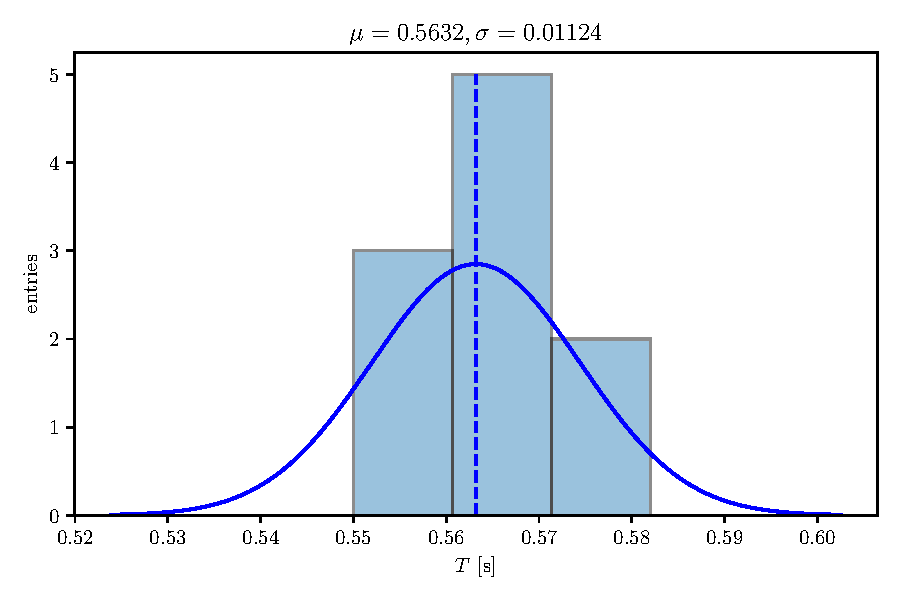
\includegraphics[width=\textwidth]{Images/Histo_T4.pdf}
    \caption{Periodo singola oscillazione 4 dischi.}
  \end{minipage}%
  \begin{minipage}{0.5 \textwidth}
    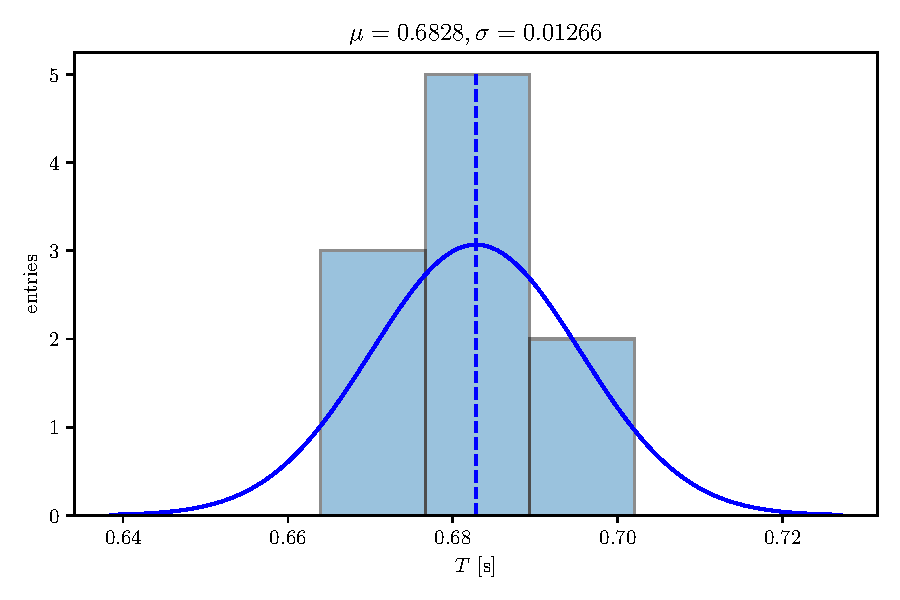
\includegraphics[width=\textwidth]{Images/Histo_T6.pdf}
    \caption{Periodo singola oscillazione 6 dischi.}
  \end{minipage}
\end{figure}

\begin{figure}[ht]
  \centering
  \begin{minipage}{0.5 \textwidth}
    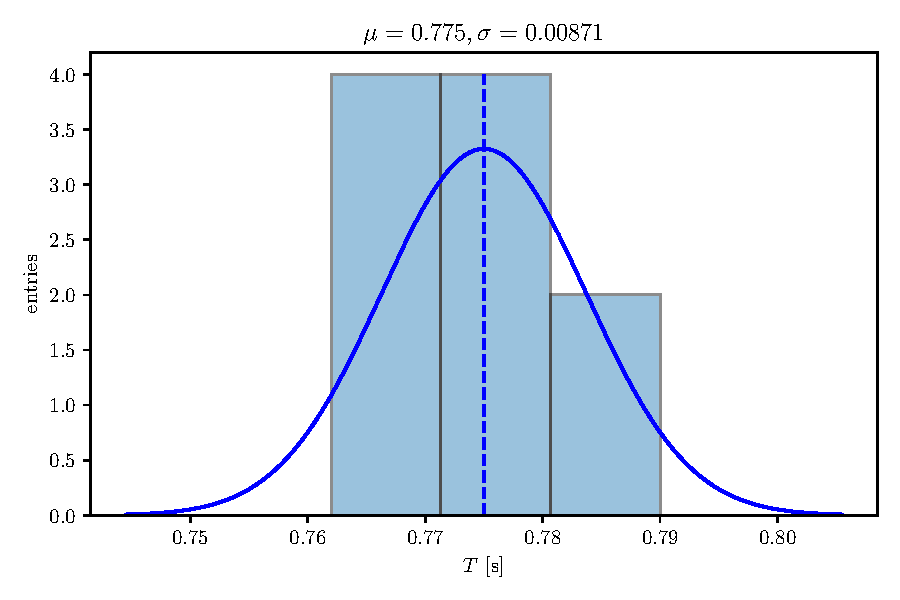
\includegraphics[width=\textwidth]{Images/Histo_T8.pdf}
    \caption{Periodo singola oscillazione 8 dischi.}
  \end{minipage}%
  \begin{minipage}{0.5 \textwidth}
    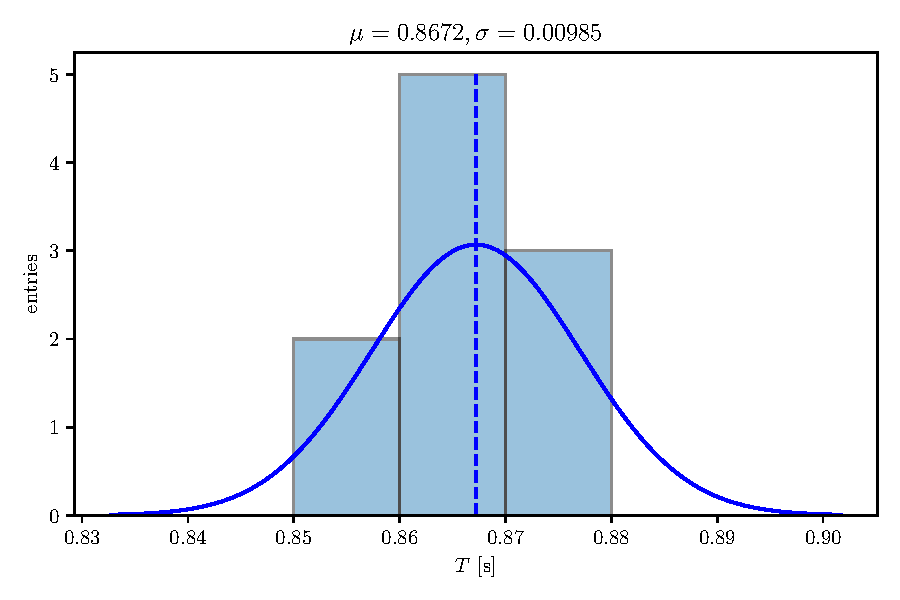
\includegraphics[width=\textwidth]{Images/Histo_T10.pdf}
    \caption{Periodo singola oscillazione 10 dischi.}
  \end{minipage}
\end{figure}

%---------------------------------------------
\subsection{Misura di \texorpdfstring{$k$}{k}}

\begin{table}[ht]
  \centering
  \begin{tabular}{rcccc}
    \toprule
    & valore & $\sigma$ & unità \\
    \midrule
    $k$ & 42.7 & 4.3 & \si{\newton\per\metre} \\
    \bottomrule
  \end{tabular}
  \caption{Risultato finale per la costante elastica della molla $k$ con la corrispondente incertezza.}
\end{table}

\pagebreak
%---------------------------------------------
\subsection{Misura di \texorpdfstring{$g$}{g}}

Stimando in maniere preliminare il coefficiente angolare impostando $\sigma_x = 0$ si ottiene $\alpha = 23.3696971$. Usando questo $\alpha$ per calcolare le $\sigma_{Y_i}$ e ripetendo il fit lineare si ottengono i seguenti valori:

\begin{figure}[ht]
  % Fit
  \begin{minipage}{0.55 \textwidth}
    \includegraphics[width=\textwidth]{example-image}
    \caption{Fit lineare.}
  \end{minipage}
  \hfill
  % Table
  \begin{minipage}{0.4 \textwidth}
    \begin{tabular}{lll}
      \toprule
      & valore & unità \\
      \midrule
      $\overline{x}$             & 0.55985438   & \si{\second\squared} \\
      $\overline{y}$             & 18.56827978  & \si{\centi\metre} \\
      $\overline{x^2}$           & 0.33791517   & \si{\second\tothe{4}} \\
      $\overline{xy}$            & 10.96705875  & \si{\second\squared\centi\metre} \\
      Var$[x]$                   & 0.02447825   & \si{\second\tothe{4}} \\
      Cov$[x,y]$                 & 0.57152617   & \si{\second\squared\centi\metre} \\
      $\sum_i \sigma_{y_i}^{-2}$ & 671.00945559 & \si{\per\centi\metre\squared} \\
      \bottomrule
    \end{tabular}
    \caption{Quantità utilizzate come input nel fit lineare. $y = x_{eq}$, $x = T^2$, $\sigma_{y_i}$ = incertezze \underline{finali} associate alle $y_i$ tenendo conto anche delle incertezze sulle $x_i$.}
  \end{minipage}
\end{figure}

\begin{figure}[ht]
  \centering
  \begin{minipage}{0.5 \textwidth}
    \includegraphics[width=\textwidth]{example-image-a}
    \caption{Residui.}
  \end{minipage}%
  \begin{minipage}{0.5 \textwidth}
    \includegraphics[width=\textwidth]{example-image-b}
    \caption{Residui standardizzati.}
  \end{minipage}
\end{figure}

\begin{table}[ht]
  \centering
  \begin{tabular}{llll}
    \toprule
    & valore & $\sigma$ & unità \\
    \midrule
    $\alpha$ & 23.35 & 0.25 & \si{\centi\metre\per\second\squared} \\
    $x_0$    & 5.50  & 0.14 & \si{\centi\metre} \\
    \bottomrule
  \end{tabular}
  \caption{Risultato del fit lineare $x_{eq} = \alpha T^2 + x_0$. Migliori stime dei parametri $\alpha$ e $x_0$ con le relative incertezze.}
\end{table}

\pagebreak

\begin{table}[ht]
  \centering
  \begin{tabular}{rcccc}
    \toprule
    & valore & $\sigma$ & unità \\
    \midrule
    $g$ & 9.2 & 0.1 & \si{\metre\per\second\squared} \\
    \bottomrule
  \end{tabular}
  \caption{Risultato finale per l'accelerazione di gravità $g$ con la corrispondente incertezza.}
\end{table}

%--------------------------------------------------------------------------------
\subsubsection{Considerazioni sul valore sperimentale di \texorpdfstring{$g$}{g}}

\begin{equation*}
  z = \frac{|g - g_{Roma}|}{\sigma_g} = 6.03066
\end{equation*}
È evidente un elevata discrepanza dal valore aspettato. Questo è dovuto probabilmente a diversi fattori: il tempo di reazione durante le misure dei periodi, la non perfetta oscillazione verticale della molla e la non perfetta lettura delle $x_{eq}$ dovuta ad un probabile errore di parallasse (nonostante l'utilizzo della squadra).

\end{document}
